\documentclass{article}
\usepackage{graphicx}
\usepackage{amsmath}

\graphicspath{ {./images/} }

\newcommand{\vect}{\overset{\rightharpoonup}}

\begin{document}

\section{Introduction}
This report covers the work done in modeling the phenomenon of leapfrogging vortex rings. This takes place when a vortex ring is close enough to another so that they affect the velocity and path of one another. Under the right circumstances, the two vortex rings can leapfrog one another, with one vortex ring being pulled through the other and then continuing on, and then repeating the process. Using the equations that have been derived to calculate induced velocity due to a vortex, I was able to write a program that models the leapfrogging vortex rings phenomenon.

\section{Methodology}
The equation for the induced velocity due to a vortex is

\begin{figure}[h!]
    \centering
    \[\vect{V} = \frac{\vect{\Gamma}\times\vect{r}}{2\pi r^2}\]
    \caption{Induced velocity}
    \label{eqn:velocity}
\end{figure}

In this equation, $\vect{r}$ is the distance vector from the point in question to the vortex, r is the magnitude of that vector, and $\vect{V}$ is the strength of the vortex (in vector form). To continue, the 2-dimensional cross section of the 2 ring vortexes had to be used, forming 4 different sections (see figure \ref{fig:vortexes}). The variable d in figure \ref{fig:vortexes} represents the distance between sections.

\begin{figure}
\centering
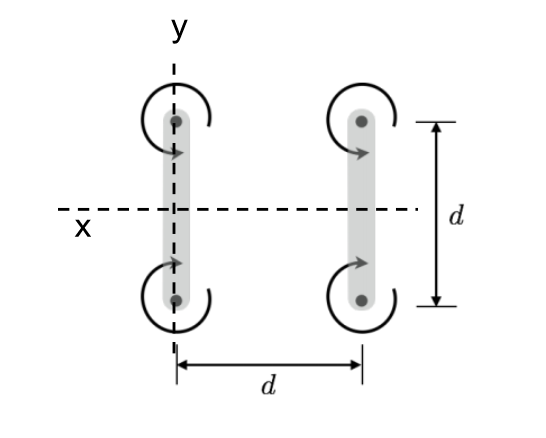
\includegraphics{vortexes}
\caption{Ring vortexes in 2-D plane}
\label{fig:vortexes}
\end{figure}

I then created a function to calculate induced velocity using the above equation. It took in the position of what section of what vortex that the induced velocity is being calculated for, the strength of the vortexes (\(\Gamma\)), and the positions of the other three sections (because we are looking at the 2-dimensional cross section of the 2 ring vortexes, there are four sections that we are calculating for. See figure \ref{fig:vortexes}). It is also important to note that the positions of the 4 different sections is all relative to however the coordinate plane is oriented. I set the x-axis to be directly in the middle of the top and bottom sections and the y-axis to be through the left 2 sections (See figure \ref{fig:vortexes}). Using these parameters, I calculated the induced velocity on the section of the vortex in question from the three other sections. I then added those three induced velocities together to get the total induced velocity on the section of the vortex in question. It is important to note that the induced velocities of the bottom sections had to be multiplied by a factor of -1 in order to be accurate, since their vorticity is negative.

Continuing, the total induced velocity could then be multiplied by a small time interval to approximate the position of the vortex after that time. So, after calculating the position of each vortex after the small time interval, the whole process is repeated with the new positions of the 4 different sections. This is continued for as many steps of time you want. All of the position data was then used to plot the paths of the vortexes, which shows the leapfrogging ring vortexes phenomenon.

\section{Results}
After running the program that computes and models the paths of the leapfrogging vortexes, I was able to see how adjusting the values of the passed parameters altered what the modeled paths looked like. I first passed the suggested values, which was a distance (d) of 1.0 meter, a strength vector of [0,0,1], 4000 time steps, and a time interval of 0.01 seconds. This produced a plot that shows clearly the leapfrogging vortex phenomenon (see figure \ref{fig:paths_01_time}).

\begin{figure}[ht]
\centering
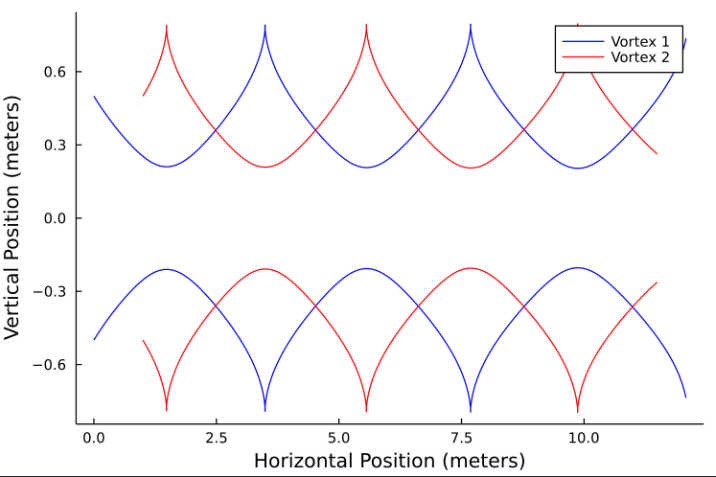
\includegraphics[scale=0.75]{images/plots_1.1.4000.01.png}
\caption{Paths of leapfrogging vortexes}
\label{fig:paths_01_time}
\end{figure}

I then chose to alter the time interval parameter to see how it affected the plot. The values I chose to use were 0.05, 0.1, and .5 seconds to show the plot changes when the time interval is increased (see figures \ref{fig:paths_05_time}, \ref{fig:paths_1_time}, and \ref{fig:paths_5_time}, respectfully).

\begin{figure}[ht]
\centering
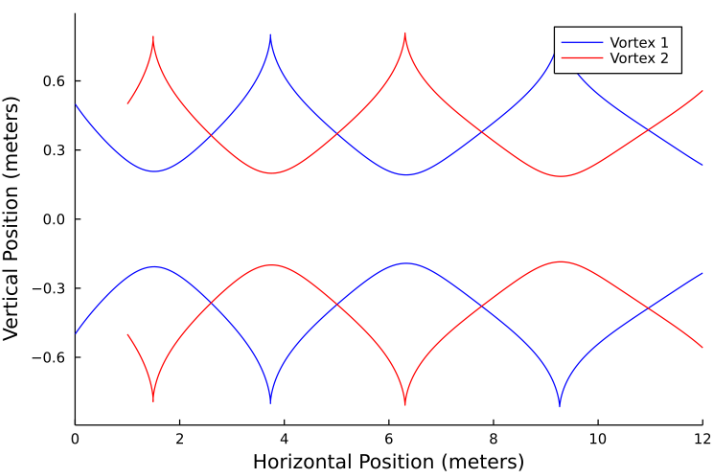
\includegraphics[scale=.75]{images/plots_1.1.4000.05.png}
\caption{Paths with 0.05 second interval}
\label{fig:paths_05_time}
\end{figure}

\begin{figure}[ht]
\centering
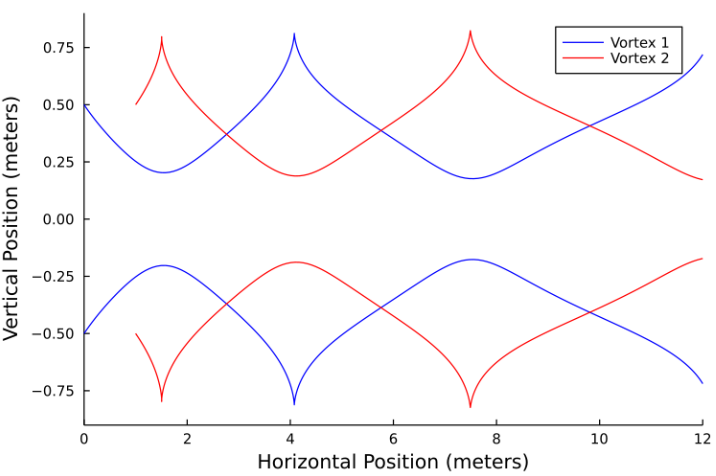
\includegraphics[scale=0.75]{images/plots_1.1.4000.1.png}
\caption{Paths with 0.1 second interval}
\label{fig:paths_1_time}
\end{figure}

\begin{figure}[ht]
\centering
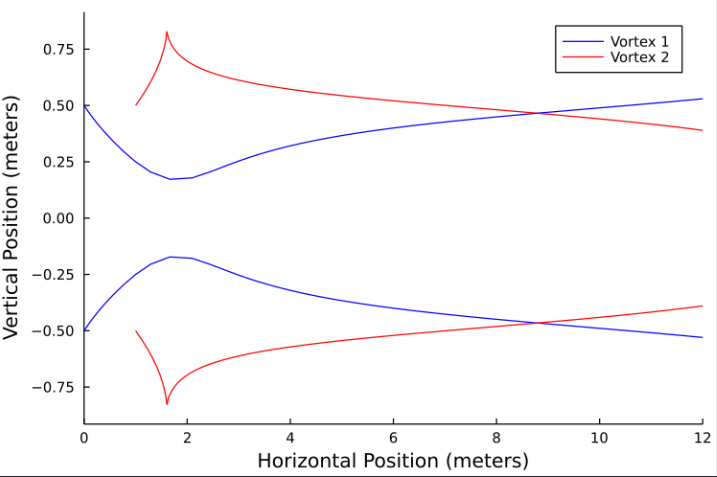
\includegraphics[scale=0.75]{images/plots_1.1.4000.5.png}
\caption{Paths with 0.5 second interval}
\label{fig:paths_5_time}
\end{figure}

These plots show that as the time interval gets larger, the vortex rings leapfrog each other slower and slower. Of course, this increasing of the time interval doesn't actually have any real-life application, as it is only used in calculating the approximation of what the paths will look like. So in reality, as the time interval used gets larger and larger, the less accurate the plots become (see figure \ref{fig:paths_5_time}).

Another parameter that I decided to alter was the distance between vortex rings. The values I chose to use were 0.5 and 1.5 meters so that could see how the plots looked when the distance between vortexes was decreased and increased (see figures \ref{fig:paths_.05_distance} and \ref{fig:paths_1.5_distance}).

\begin{figure}[ht]
\centering
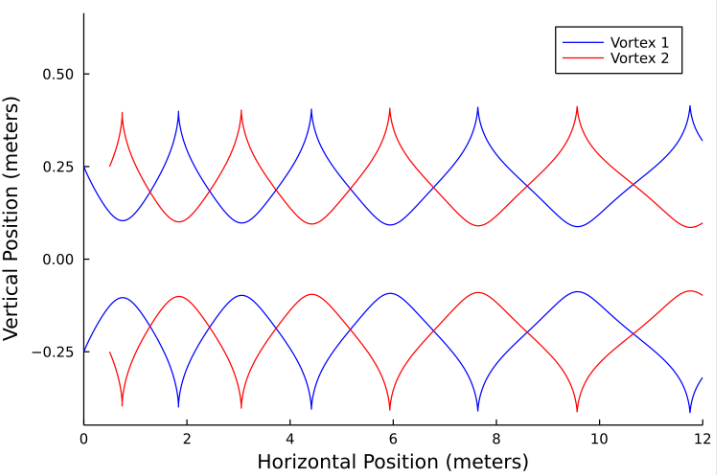
\includegraphics[scale=0.75]{images/plots_.05.1.4000.01.png}
\caption{Paths when d=0.05 meters}
\label{fig:paths_.05_distance}
\end{figure}

\begin{figure}[ht]
\centering
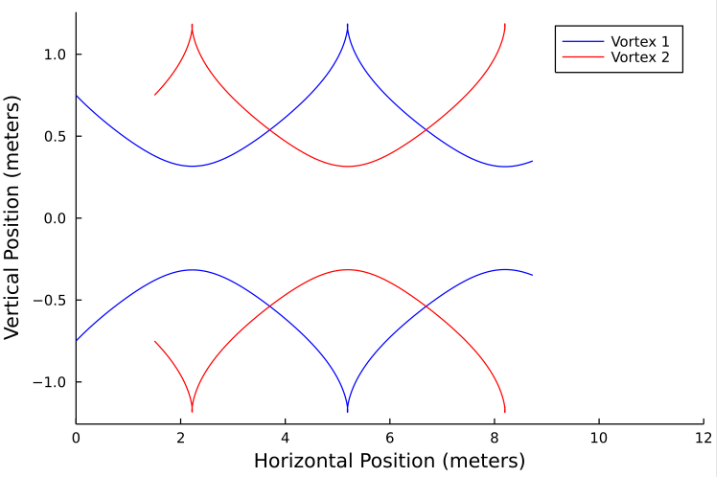
\includegraphics[scale=0.75]{images/plots_1.5.1.4000.01.png}
\caption{Paths when d=1.5 meters}
\label{fig:paths_1.5_distance}
\end{figure}

From these figures, we see that when the distance between vortexes is decreased, the vortexes leapfrog each other much quicker (see figure \ref{fig:paths_.05_distance}). When the distance is increased, the leapfrogging action is slowed (see figure \ref{fig:paths_1.5_distance}). This is when being compared to the paths in figure \ref{fig:paths_01_time}.

\end{document}
